


The problem is to optimize and parallelize a particle simulator, we
were given four implementations of the simulator:

\begin{wrapfigure}{r}{0.3\textwidth}
    \vspace{-130pt}
    \begin{center}
        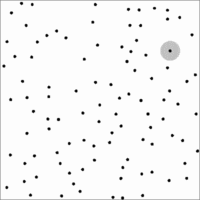
\includegraphics[width=0.28\textwidth]{simulator}
    \end{center}
    \caption{An example simulation in the provided visualizer application.}
\end{wrapfigure}

\begin{itemize}
     \item One running sequentially
     \item One parallelized using pthreads
     \item One parallelized using openmp 
     \item One parallelized using MPI
\end{itemize}

The given simulator implementation used $n^2$ computations each frame, where $n$ is the number of particles.

In contrast to the traditional N-body problem this simulation only
simulates the interaction between particles within a certain distance from
each other, moreover the density of particles is set low enough so that
only $O(n)$ interactions are expected at any given moment. Therefore it
should be possible to do the necessary calculations for each frame in
$O(n)$. The first task at hand is to make this optimization, since the given code runs in $O(n^2)$.

The second task is to use different parallelizing techniques to achieve a near optimal speedup factor. In other words, the program should run in $O(n)/T$ time, where $T$ is the number of threads.
